
% ---------------------------
% Lista delle sezioni
% ---------------------------

% - una sezione introduttiva con la descrizione degli algoritmi e delle scelte implementative che avete fatto;
% - grafici esplicativi dei risultati con le risposte alle due domande;
% - eventuali originalità introdotte nell'elaborato o nell'implementazione;
% - una sezione conclusiva in cui porre i vostri commenti e le vostre conclusioni sull’elaborato svolto e i risultati ottenuti.
% - (A PARTE) Il codice sorgente dell’implementazione in un unico file di archivio (.zip, .tar.gz, ecc.).
% Note generali (ultima sezione)


% Start counting pages
\pagenumbering{arabic}
\clearpage
\setcounter{page}{1}

% Introduzione 
\newpage
\section{Introduzione}

\subsection{Descrizione del problema}

In questa relazione illustreremo dei confronti tra tre algoritmi per risolvere un problema
intrattabile, confrontando i tempi di calcolo e la qualità delle soluzioni
che si possono ottenere con \textbf{algoritmi esatti} e con \textbf{algoritmi di approssimazione}.
Il problema in questione è il \textbf{Travelling Salesman Problem} (\textbf{TSP} o
\textit{Problema del Commesso Viaggiatore}). Il nome di questo problema deriva dalla sua
definizione: data una rete di città, connesse tra loro tramite strade, si determini il
percorso di minore distanza che un commesso viaggiatore deve fare per visitare tutte le città
\underline{una e una sola volta}.

Il \textit{TSP} si può rappresentare con un grafo non orientato, pesato e
completo $G = (V,E)$, dove i vertici sono le città e il peso del lato $(u,v)$
è uguale alla distanza da $u$ a $v$. Risolvere il \textit{TSP} significa trovare un
\textbf{circuito Hamiltoniano}, ovvero un ciclo di costo minimo che visita tutti
i vertici \textit{esattamente una volta}.

\subsection{NP-completezza del problema}

\subsubsection{Dimostrazione di NP-completezza}

Prima di tutto dimostriamo che TSP $\in \mathcal{NP}$. Data un'istanza del problema, usiamo
come \textit{certificato} la sequenza degli $n$ vertici del ciclo di peso minimo.
L'algoritmo di verifica del certificato deve controllare che la sequenza contenga ogni
vertice di $G$ esattamente una volta, sommare il peso dei lati e controllare che il peso
totale del ciclo sia inferiore a $k$. Questo controllo si può svolgere in tempo polinomiale
($O(n)$).

Per poter stabilire con precisione la complessità del problema, è necessario prima
“trasformare” tale problema in un \textit{problema di decisione}, aggiungendo un limite $k$
per il peso del ciclo all'input del problema.

\textbf{Definizione di TSP decisionale}: Dato un grafo non orientato, completo e pesato
$G = (V,E)$ e un valore $k > 0$, esiste un ciclo in $G$ che attraversa tutti i vertici una
sola volta di peso inferiore a $k$.

\textbf{Teorema}: \textit{TSP} è un problema $\mathcal{NP}$-completo.

\textit{Dimostrazione}: è già stato dimostrato che \textit{TSP} $\in \mathcal{NP}$, quindi si procede nel dimostrare
che \textit{TSP} è $\mathcal{NP}$-hard. Si mostra quindi una riduzione del problema del circuito Hamiltoniano a TSP.
Prendiamo un grafo non orientato $G = (V,E)$ e costruiamo un'istanza di \textit{TSP} che ci permetta di risolvere
il problema del circuito Hamiltoniano su $G$. Costruiamo un grafo non orientato e completo $G' = (V, E')$
con gli stessi vertici di $G$ e $E' = \{(u, v) | u, v \in V\}$. Il peso degli archi di $G'$ viene assegnato
come segue

\[
    w(u, v) = 0, \textnormal{ se } \{u, v\} \in E
\]
\[
    w(u, v) = 1, \textnormal{ se } \{u, v\} \notin E
\]

È possibile notare che si può costruire il grafo $G'$ in tempo polinomiale rispetto al numero
di vertici $|V|$ del grafo di partenza $G$. Il grafo $G$ contiene un circuito Hamiltoniano se e
solo se $G'$ ha un ciclo di peso minore o uguale a 0. Supponiamo che $G$ contenga un circuito
Hamiltoniano $h = v_1, \dots, v_n$. Ogni lato che compone $h$ è presente in $E$ e quindi ha peso 0 in $G'$.
Di conseguenza, $h$ è un ciclo di $G'$ di peso uguale a 0. Viceversa, supponiamo che $G'$ contenga un ciclo
semplice $t$ che attraversa tutti i vertici di peso minore o uguale a 0. Poiché i pesi dei lati
in $G'$ sono solo 0 oppure 1, tutti i lati che compongono $t$ devono avere costo 0. Quindi tutti i
lati del ciclo sono presenti anche in $E$ e $t$ è un circuito Hamiltoniano per $G$. $ \square $

\subsubsection{Inapprossimabilità per fattori $\rho$ costanti di TSP}

Il \textit{TSP} è un problema simile al problema del MST: il MST è un cammino di peso minimo
che collega tutti i vertici del grafo $G$, mentre il \textit{TSP} è un ciclo di peso minimo
che collega tutti i vertici del grafo $G$. Nonostante questa somiglianza tra questi
due problemi, il \textit{TSP} è un problema molto difficile anche solo da approssimare. Se
esistesse un algoritmo di approssimazione con un $\rho$ costante, allora si saprebbe
risolvere in tempo polinomiale un problema \textit{$\mathcal{NP}$-hard}.

\textbf{Teorema}: se $\mathcal{P} \ne \mathcal{NP}$, non può esistere alcun algoritmo
(polinomiale) di $\rho$-approssimazione per \textit{TSP} con $\rho = \mathcal{O}(1)$.

\textit{Dimostrazione}: per assurdo, si supponga che esista un algoritmo $A_\rho$
polinomiale di $\rho$-approssimazione per \textit{TSP}. Si dimostra come costruire $A_{Hamilton}$
che decide il problema del ciclo Hamiltoniano in tempo polinomiale. Sia $I = G =(V,E)$
e $O = $ "$G$ contiene un ciclo Hamiltoniano?". Si effettua quindi una \textit{riduzione}:
\[
    G \rightarrow G' = (V, E') \textnormal{ è completo, dove }
\]
\[
    c(e \in E') = 1 \textnormal{ se } e \in E \textnormal{, altrimenti } c(e \in E') = \rho|V| + 1
\]

Possiamo quindi creare delle rappresentazioni di $G'$ e di $c$ a partire dalle rappresentazioni
di $G$ in tempo polinomiale in $|V|$ ed $|E|$.

Eseguo $A_\rho(G') \rightarrow C \textnormal{ (ciclo), } c(C) \textnormal{(funzione di costo di $C$, $c: V \times V \rightarrow \mathcal{N}$)}$ e si
determina:
\begin{enumerate}
\item $G \in HAMILTON \Rightarrow c(C^*) = |V| \Rightarrow A_\rho$, ritorna un ciclo $C$
con $c(C) \le \rho|V|$;
\item $G \not\in HAMILTON \Rightarrow C$ contiene almeno un lato non in
$G$ (più precisamente in $E$) $\Rightarrow c(C) \ge \rho|V| + 1$. Poiché i lati che non
appartengono a $G$ sono costosi, c'è un \textit{gap} di almeno $\rho |V|$ tra il costo di un cammino
che è Hamiltoniano in $G$ (di costo $|V|$) e il costo di qualsiasi altro cammino (di costo
almeno $\rho |V| + |V|$). Pertanto, il costo di un cammino che non è un ciclo Hamiltoniano
in $G$ è almeno un fattore $\rho + 1$ maggiore del costo di un cammino che è un ciclo
Hamiltoniano in $G$.
\end{enumerate}

È possibile notare che si può costruire il grafo $G'$ in tempo polinomiale rispetto al numero
di vertici $|V|$ del grafo di partenza $G$. Il grafo $G$ contiene un circuito Hamiltoniano se e
solo se $G'$ ha un ciclo di peso minore o uguale a 0. Supponiamo che $G$ contenga un circuito
Hamiltoniano $h = v_1, ..., v_n$. Ogni lato che compone $h$ è presente in $E$ e quindi ha peso 0 in $G'$.
Di conseguenza, $h$ è un ciclo di $G'$ di peso uguale a 0. Viceversa, supponiamo che $G'$ contenga un ciclo
semplice $t$ che attraversa tutti i vertici e di peso minore o uguale a 0. Poiché i pesi dei lati
in $G'$ sono solo 0 oppure 1, tutti i lati che compongono $t$ devono avere costo 0. Quindi tutti i
lati del ciclo sono presenti anche in $E$ e $t$ è un circuito Hamiltoniano per $G$. $\square$

\label{tsp_metrico}
\subsection{TSP metrico}

Istanza particolare \textit{TSP} in cui l'input, in particolare la funzione di costo $c$, soddisfa la
\textbf{disuguaglianza triangolare}:
\[
\forall u, v, w \in V, \textnormal{ vale che } c(u, v) \le c(u, w) + c(w, v) \Rightarrow
c(<u, v>) \le c(<u, w, v>)
\]

dove $c$ è la \textit{funzione di costo}. Secondo questa definizione, per ogni insieme di tre nodi
possibili del grafo $G$, vale che il costo di un lato $(u, v)$ è al più il costo di un lato $(u, w)$
più il costo di un lato $(w, v)$. Questo significa che il costo del cammino per andare da $u$ a $v$
attraverso l'unico lato che li collega è più conveniente del cammino per andare da $u$ a $w$ e da
$w$ a $v$. Chiamiamo questo problema \textbf{TRIANGLE\_TSP}. Questa restrizione del problema
$\mathcal{NP}$-completo si trova in $\mathcal{P}$.

% \textbf{Teorema}: 

% Descrizione degli algoritmi
\newpage
\section{Descrizione degli algoritmi}

\subsection{Struttura dati per il grafo}

Per comodità nell'implementazione abbiamo realizzato due diverse strutture dati per rappresentare un multigrafo; queste sono simili tra loro ma presentano alcune differenze.

\subsubsection{Struttura dati per Stoer-Wagner}
Per quanto riguarda la struttura dati per l'esecuzione dell'algoritmo Stoer-Wagner, un oggetto \texttt{Graph} è rappresentato nel seguente modo:

\begin{enumerate}
    \item \verb|V| è un insieme di nodi;
    \item \verb|E| è una lista di lati;
    \item \verb|Graph| rappresenta la \textit{lista di adiacenza}.
    Gli indici per accedere alla mappa sono rappresentati dai vertici.
    Ogni cella della mappa punta ad una lista di coppie di valori
    (il vertice a cui è collegato e il peso del lato che li
    congiunge);
    \item \verb|totalVertex| rappresenta il numero di vertici;
    \item \verb|totalEdges| rappresenta il numero di archi;
    \item \verb|datasetName| rappresenta il nome del grafo.
\end{enumerate}
Essendo l'oggetto in questione un multigrafo, la lista di adiacenza e la lista di lati possono contenere più archi tra due nodi aventi pesi diversi.

\noindent I metodi implementati sono:
\begin{enumerate}
    \item \verb|add_vertex|: aggiunge un vertice al grafo;
    \item \verb|add_edge|: aggiunge un lato al grafo;
    \item \verb|remove_edge|: rimuove un lato dal grafo;
    \item \verb|remove_node|: rimuove completamente un vertice dal grafo, ossia rimuove il vertice dalla relativa lista e tutti gli archi a esso collegati;
    \item \verb|totalWeightCost|: restituisce la somma di tutti i lati tra due vertici.
\end{enumerate}

\subsubsection{Struttura dati per Karger-Stein}
\label{struttura_dati_karger_stein}
La struttura dati per quanto riguarda l'algoritmo di Karger-Stein (\verb|KargerGraph|) contiene i seguenti campi:
\begin{enumerate}
  \item \verb|n_edges|: rappresenta il numero di lati del grafo;
  \item \verb|n_vertices|: rappresenta il numero di vertici del grafo;
  \item \verb|W|: rappresenta la \textit{matrice di adiacenza} del grafo;
  \item \verb|D|: rappresenta il vettore dei \textit{gradi pesati} dei vertici del grafo (successivamente verrà illustrato 
  il motivo dell'utilità di questa struttura).
\end{enumerate}

I metodi implementati per questa struttura dati sono:
\begin{enumerate}
  \item \verb|add_edge|: aggiunge un lato al grafo;
  \item \verb|remove_edge|: rimuove un lato al grafo;
  \item \label{calculate_weighted_degrees_vertices} \verb|calculate_weighted_degrees_vertices|: permette di calcolare i gradi pesati dei vertici. Tali risultati vengono 
  memorizzati in \verb|D|.
\end{enumerate}

\subsection{Stoer e Wagner}

\subsubsection{Introduzione}

L'algoritmo di Stoer-Wagner è un algoritmo ricorsivo per la risoluzione del problema del minimum cut di grafi non diretti, pesati e con pesi degli archi non negativi. Questo algoritmo è di tipo deterministico, ossia non vi è alcuna componente di randomicità in esso. \\
L'idea base dell'algoritmo è la seguente: 
\begin{itemize}
  \item A ogni fase, l'algoritmo trova un \textit{s-t minimum cut} tra due vertici;
  \item L'algoritmo contrae quindi il grafo rispetto all'arco $\{s,t\}$ al fine di ricercare un taglio diverso da \textit{s-t};
  \item Il taglio di peso minimo trovato in tutte le iterazioni dell'algoritmo è il risultato dell'algoritmo, e coincide con il \textit{minimum cut} del grafo.
\end{itemize}

\subsubsection{Algoritmo}

L'algoritmo è composto da due funzioni:
\begin{itemize}
  \item \texttt{GlobalMinCut}: funzione ricorsiva che si occupa di chiamare \texttt{stMinCut} e di restituire il \textit{minimum cut} globale di peso minore;
  \item \texttt{stMinCut}: funzione che si occupa di trovare un \textit{s-t minimum cut}.
\end{itemize}

Viene qui riportato lo pseudocodice per entrambe le funzioni.

\begin{verbatim}
  function GlobalMinCut(G=(V,E,w))
    if V = {a,b} then
      return({a}, {b})
    else
      (C1, s, t) <- stMinCut(G)
      C2 <- GlobalMinCut(G/{s,t})
      if w(C1) <= w(C2) then
        return C1
      else
        return C2
\end{verbatim}

\begin{verbatim}
  function stMinCut(G=(V,E,w))
    A <- {a}
    while A != V do
      trova v in V che massimizza w(A,{v})
      A <- A unito {v}
    siano s e t gli ultimi due vertici aggiunti ad A
    return (V-{t},{t}), s, t
\end{verbatim}

Poiché la ricerca del nodo che massimizza w(A,{v}) può essere un'operazione computazionalmente pesante, complice anche la necessità di iterare sull'intera lista di nodi, l'algoritmo può essere facilmente ottimizzato tramite l'utilizzo di una coda di priorità; questa infatti permette di ottenere il nodo di peso massimo in tempo costante. La funzione \texttt{stMinCut} può essere quindi modificata come segue.

\begin{verbatim}
  function stMinCut(G=(V,E,w))
    Q <- empty
    for all u in V do
      key[u] <- 0
      Insert(Q, u, key[u])
    s, t <- null
    while Q != empty do
      u <- ExtractMax(Q)
      s <- t; t <- u
      for all (u,v) in E do
        if v in Q then
          key[v] <- key[v] + w(u,v)
          IncreaseKey(Q, v, key[v])
    return (V-{t},{t}), s, t
\end{verbatim}

La complessità dell'algoritmo è fortemente legata alla struttura dati che viene utilizzata. La funzione \texttt{stMinCut}, infatti, ha complessità $O(mlogn)$ se implementata tramite \textit{MaxHeap} e $O(m+nlogn)$ se implementata tramite \textit{Fibonacci Heap}. \\
Di conseguenza la funzione \texttt{GlobalMinCut}, e quindi l'algoritmo, ha complessità $O(mnlogn)$ se implementato tramite \textit{MaxHeap} e $O(mn+n^2 logn)$ se implementato tramite \textit{Fibonacci Heap}. Nel caso specifico della nostra implementazione, avendo usato la struttura dati \textit{MaxHeap}, ci attendiamo che la complessità teorica sia $O(mnlogn)$.

\subsubsection{Implementazione}

Per implementare l'algoritmo Stoer e Wagner in Python abbiamo realizzato una classe denominata \texttt{StoerWagner} che definisce una serie di metodi per la corretta esecuzione dell'algoritmo.
Nello specifico: 

\begin{itemize}
    \item \texttt{algorithm}, che si occupa di mandare in esecuzione \texttt{globalMinCut} sul grafo di input;
    \item \texttt{stMinCut}, che cerca un min cut (S,T) sfruttando un \textit{max-heap} come \textit{priority queue} da cui estrarre i nodi con peso dei lati maggiori, individuando così i vertici s e t da ritornare;
    \item \texttt{globalMinCut}, che esegue la ricerca ricorsivamente di un min cut globale a partire dal grafo di input e, nel caso in cui il grafo contenga solo due nodi, restituisca come caso base i nodi presenti come tupla.
    \item \texttt{weightMinCut}, usato per ritornare il peso del vertice in input a partire dai pesi dei lati;
    \item \texttt{contractGraph}, usato contrarre il grafo in modo iterativo rispetto ai vertici \textit{s} e \textit{t} in input. 
\end{itemize}

Le implementazioni fanno uso della struttura dati \texttt{graph} precedentemente menzionata, attraverso cui viene costruita la matrice di adiacenza, nonché il vettore di vertici del grafo in input. Rispetto a quanto riportato nello pseudocodice, inoltre, abbiamo fatto uso delle tuple conservare i pesi calcolati con \texttt{key[v]} per i singoli vertici, che poi vengono recuperati da \texttt{weightMinCut} per ritornare il peso del min cut, senza necessità di doverlo ricalcolare.

\subsubsection{Ottimizzazioni implementate}

Per quanto concerne le ottimizzazioni, abbiamo evitato - a meno della prima e unica invocazione di \texttt{algorithm} - la copia profonda di tutto \texttt{Graph}, preferendo la sola copia della lista di vertici, dal momento che questa era quella maggiormente soggetta ad alterazioni. La lista di vertici è stata poi constantemente passata tra i vari metodi di classe e questo ci ha velocizzato in buona parte il passaggio di variabili, nonché ridotto il tempo totale di esecuzione dell'algoritmo stesso. Inoltre, abbiamo preferito l'uso della copia profonda manuale rispetto a quella di sistema, inserendo gli \(n-1\) vertici in una nuova lista, poi passata come risultato dei metodi. 
Al fine di velocizzare la parte di aggiornamento dei pesi dei nodi nel \textit{max-heap}, abbiamo riscritto la funzione \texttt{searchAndUpdateWeight} in \texttt{increaseKey} come metodo a sé stante, garantendo così la riduzione di una buona percentuale di tempo impiegato per l'aggiornamento del peso dei nodi. Inoltre, sempre nel \textit{max-heap}, abbiamo recuperato una vecchia ottimizzazione consistente nell'utilizzo di una mappa, concretizzata in una variabile di tipo \texttt{defaultdict} in Python, che associa a ogni nodo la sua posizione in \textit{list}, ossia la lista dei nodi. Questa implementazione permette di ricercare la presenza di un vertice nello Heap in tempo costante, e ciò è particolarmente utile perché la presenza del vertice deve essere verificata due volte ad ogni iterazione del ciclo for dell'algoritmo (nella condizione if e durante l'aggiornamento dello heap). Se non avessimo adottato tale ottimizzazione, queste operazioni avrebbero avuto una complessità lineare, andando così ad aumentare polinomialmente la complessità computazionale dell'algoritmo.
L'insieme di tutte queste piccole ottimizzazioni ci ha permesso di non dover inserire una soglia di tempo massima entro cui l'algoritmo doveva eseguire.
\subsection{Karger e Stein}
\label{karger_stein_section}

\subsubsection{Introduzione all'algoritmo di Karger}
I passi svolti dall'algoritmo di Karger sono:
\begin{enumerate}
    \item Viene scelto a caso un lato;
    \item Si \textit{contraggono} (si veda \ref{definizione_contrazione}) i due vertici 
    relativi, eliminando tutti i lati incidenti su entrambi;
    \item Si ripetono questi due passi finchè restano solo \textit{due} vertici;
    \item Quando sono rimasti soltanto due vertici, si restituiscano i lati che  
    connettono i due vertici.
\end{enumerate}

\subsubsection{Introduzione all'algoritmo di Karger-Stein}
L'algoritmo di Karger-Stein è un algoritmo randomizzato ricorsivo che fa parte della 
categoria di algoritmi Monte Carlo. La versione di questo algoritmo è in grado di 
offrire delle prestazioni migliori rispetto all'algoritmo di Karger e può essere 
applicato per grafi pesati (si veda la descrizione del problema 
\ref{descrizione_min_cut}). Per fare ciò, l'operazione di \verb|full_contraction| 
deve essere ridefinita, in modo tale che:
\begin{enumerate}
    \item Deve essere scelto un lato con probabilità proporzionale al peso del lato 
    \item stesso;
    \item Sia possibile scegliere il lato da contrarre in tempo lineare;
    \item Effettuare la contrazione in tempo lineare.
\end{enumerate}

Riprendendo quanto illustrato precedentemente (si veda 
\ref{struttura_dati_karger_stein}), la struttura dati \verb|KargeGraph| 
include al suo interno altre due strutture dati:
\begin{enumerate}
    \item La matrice di adiacenza \textit{pesata} \verb|W|
    $n \times n$, tale che: 
    \[
        W[u,v] = w(u,v) \textnormal{ se } (u,v) \in \mathcal{E} 
        \textnormal{, altrimenti } 0
    \]
    \item Il vettore dei \textbf{gradi pesati} dei vertici:
    \[
        D[u] = \sum_{v \in \mathcal{V}} W[u,v]
    \]
\end{enumerate}

La procedura di \verb|full_contraction| viene scomposta in due fasi: 
nella prima fase viene determinato il lato e successivamente avviene la 
contrazione.

Questo algoritmo funziona con una probabilità molto bassa. Tuttavia tale probabilità 
può essere significativamente incrementata andando a ripetere questo processo un certo 
numero di volte.

L'algoritmo di Karger-Stein è composto dalle seguenti fasi:
\begin{enumerate}
    \item \textbf{Random select}
    \item \textbf{Edge select}
    \item \textbf{Contract edge}
    \item \textbf{Contract}
    \item \textbf{Recursive contract}
\end{enumerate}

\subsubsection*{Random select}
Si vuole scegliere un lato con una probabilità 
proporzionale al peso del lato stesso. Per fare ciò, si introducono i 
\textbf{pesi cumulativi}. Dati $m$ lati $e_1, e_2, \cdots , e_m$ di peso 
$w_1, w_2, \cdots , w_m$, i pesi cumulativi sono così definiti:
\[
    C[k] = \sum_{i = 1}^{k} w_i
\]
ovvero, alla posizione $k$ del \textit{vettore dei pesi cumulativi} $C$, si avrà 
la somma dei pesi dei primi $k$ lati. Quindi, in $C[m]$ si avrà la somma dei pesi 
di tutti i lati del grafo $\mathcal{G}$. A questo punto:
\begin{enumerate}
    \item Si determina un valore intero $0 \le r \le C[m]$ con 
    \textbf{probabilità uniforme};
    \item \label{scelta_lato} Si utilizza la \textit{ricerca binaria} per 
    determinare il lato $e_i$ tale che $C[i - 1] \le r \le C[i]$:
    \[
        Pr[e_i \textnormal{ viene scelto}] = Pr[C[i - 1] \le r \le C[i]] = \frac{C[i] - C[i - 1]}{C[m]} = \frac{w(e_i)}{\sum_{e \in \mathcal{E}} w(e)}
    \]
    quindi, la probabilità è il peso del lato diviso la somma dei pesi totali del 
    grafo $\mathcal{G}$. Di conseguenza, è proporzionale al peso del lato $w(e_i)$.
\end{enumerate}
L'input di questa procedura può essere un \textit{qualsiasi} vettore di pesi 
cumulativi, non necessariamente di lati.

Dal punto di vista computazionale:
\begin{enumerate}
    \item Costruzione del vettore $C$: $\mathcal{O}(m)$;
    \item Scelta del valore $r$: $\mathcal{O}(1)$;
    \item Determinare il lato $e_i$ con la ricerca binaria in $C$: 
    $\mathcal{O}(log(m))$.
\end{enumerate}
Quindi, la complessità totale di questa procedura è $\mathcal{O}(m)$. Nel caso 
peggiore, ovvero, quando il grafo è \textit{denso}, si ha $m \le \mathcal{O}(n^2)$. 
Di conseguenza la complessità di questa procedura nel caso di un grafo denso è di 
$\mathcal{O}(n^2)$. Questo risulta essere un problema, in quanto andrebbe ad 
incrementare significativamente la complessità totale dell'algoritmo. Per tale 
motivo, al posto di determinare il lato, come definito al punto \ref{scelta_lato}, 
si vuole determinare la posizione del valore $r$ nel vettore $C$.

\subsubsection*{Edge select}
Per i motivi espressi al punto 
precedente, tramite la procedura \verb|random_select| si andrà a determinare il 
vertice $u$ di partenza e poi il vertice $v$ di arrivo, in modo che la probabilità 
di scegliere un lato sia proporzionale al peso del lato stesso. La procedura 
\verb|edge_select| prende in input \verb|W| e il vettore dei gradi pesati dei 
vertici \verb|D| e svolge le seguenti operazioni:
\begin{enumerate}
    \item Si sceglie un vertice $u$ con una probabilità proporzionale a $D[u]$:
    \begin{enumerate}
        \item Si costruisce il vettore dei pesi cumulativi di $D[u]$;
        \item Viene chiamata la procedura \verb|random_select| per scegliere il 
        primo vertice;
    \end{enumerate}
    \item Si sceglie un vertice $v$ con una probabilità proporzionale a $W[u,v]$:
    \begin{enumerate}
        \item Si costruisce il vettore dei pesi cumulativi di $W[u,v]$;
        \item Viene chiamata la procedura \verb|random_select| per scegliere il 
        secondo vertice;
    \end{enumerate}
    \item Si ritorna il lato $(u,v)$.
\end{enumerate}
La complessità di questa procdeura è $\mathcal{O}(n)$ in quanto $D$ e $W[u,v]$ 
hanno una dimensione pari a $\mathcal{O}(n)$ e di conseguenza \verb|random_select| 
opererà in $\mathcal{O}(n)$ in entrambi i casi (si ricordi che \verb|W| è 
$n \times n$). Così facendo, la procedura non ha una dipendenza quadratica legata 
al numero di lati del grafo $\mathcal{G}$, ma ha una dipendenza lineare legata al 
numero di vertici del grafo $\mathcal{G}$.

\[
    Pr[(u,v) \textnormal{ scelto}] = Pr[u \textnormal{ scelto}] \cdot 
    Pr[v \textnormal{ scelto} | u] + Pr[v \textnormal{ scelto}] \cdot 
    Pr[u \textnormal{ scelto} | v]
\]
\[
    = \frac{D[u]}{\sum_v D[v]} \cdot \frac{W[u,v]}{D[u]} + \frac{D[v]}{\sum_v D[v]} 
    \cdot \frac{W[v,u]}{D[v]} =
    \frac{2 \cdot W[u,v]}{\sum_v D[v]} \textnormal{ ed è proporzionale al peso del lato } W[u,v]
\]

\subsubsection*{Contract edge}
Sulla matrice \verb|W| si va 
ad azzerare la riga e la colonna corrispondente al vertice $v$ (che verrà 
contratto). Azzerare $v$ significa \textit{eliminare} il vertice dal grafo. Si va 
ad aggiornare conseguentemente anche la matrice \verb|W| in modo da avere soltanto 
i pesi sulla matrice che corrispondono ai vertici restanti dopo la contrazione. 
Si illustra di seguito lo pseudo-codice:
\begin{verbatim}
    function contract_edge(u, v)
        D[u] = D[u] + D[v] - 2W[u,v]
        D[v] = 0
        W[u,v] = W[v,u] = 0
        for w in V, eccetto u e v do
            W[u,w] = W[u,w] + W[v,w]
            W[w,u] = W[w,u] + W[w,v]
            W[v,w] = W[w,v] = 0
\end{verbatim}
Questa procedura opera in tempo $\mathcal{O}(n)$.

\subsubsection*{Contract}
Si definisce la procedura di contrazione che opera in 
$\mathcal{O}(n^2)$. Questa procedura ritorna una contrazione di $k$ vertici del 
grafo $\mathcal{G}$ rappresentato con la matrice \verb|W| ed il vettore \verb|D|.
Si illustra di seguito lo pseudo-codice:
\begin{verbatim}
    function contract(G = (D,W), k)
        n = numero di vertici in G
        for i = 1 to n - k do
            (u,v) = edge_select(D,W)
            contract_edge(u,v)
        return D,W
\end{verbatim}

\subsubsection*{Recursive contract}


\subsubsection{Implementazione}

\subsubsection{Ottimizzazioni implementate}


% Misurazioni 
\newpage
\section{Caratteristiche del programma e Misurazioni}

\subsection{Caratteristiche del programma}

\subsubsection{Introduzione}

Il programma è stato realizzato interamente in Python e si struttura in 4 cartelle principali che rappresentano: il modulo degli algoritmi (\textit{algorithms}), il modulo delle strutture dati (\textit{data\_structures}), il modulo delle misurazioni (\textit{measurements}) e il dataset contenente i grafi (\textit{dataset}). 

\subsubsection{Installazione e requisiti}

Prima di eseguire il programma è necessario installare le dipendenze presenti nel file \textit{requirements.txt} eseguendo il seguente comando: \texttt{pip install -r requirements.txt}
\\Per l'esecuzione è richiesto l'uso di un terminale Windows, MacOs, Linux o BSD-like con Python 3.x+ e PIP installato.

\subsubsection{Avvio del programma}

Per l'esecuzione del programma è necessario spostarsi nella cartella di progetto ed eseguire il seguente comando: 
\texttt{python3 main.py [--version] [-h] <type> <dataset>} dove:

\begin{itemize}
    \item \textbf{type:} rappresenta il tipo di algoritmo o di serie di esecuzioni che si vuole avviare, nello specifico uno tra i seguenti: 
    \begin{itemize}
        \item \textit{all} (esegue e salva su file le misurazioni con le opportune ripetizioni);
        \item \textit{all-single} (esegue tutte le misurazioni singole);
        \item \textit{all-quartet} (esegue tutte le misurazioni raggruppando i grafi in base al numero di vertici, nello specifico a gruppi di quattro);
        \item \textit{sw} (esegue le misurazioni con Stoer-Wagner);
        \item \textit{ks} (esegue le misurazioni con Karger-Stein).   
    \end{itemize} 
    \item \textbf{dataset:} rappresenta una cartella contenente i file dei dataset formattati come da consegna o singolo file di dataset in input. 
    \item \textbf{--version:} è opzionale e mostra la versione del programma in esecuzione. 
    \item \textbf{-h:} è opzionale e mostra un aiuto per i comandi da utilizzare. 
\end{itemize}

\subsubsection{Caratteristiche tecniche del computer per le misurazioni} 

L'esecuzione del programma e le relative misurazioni sono state effettuate sulla seguente macchina:
\begin{itemize}
    \item \textbf{CPU:} Ryzen 9 3900x (12 core / 24 thread), 4.6ghz
    \item \textbf{RAM:} 32 GB DDR4 
    \item \textbf{SSD:} NVME SSD 512 GB
\end{itemize}

\noindent Tutte le misurazioni sono state eseguite \textbf{sequenzialmente} monitorando l'uso di un core dedicato della CPU al 100\% per tutta la durata dell'esecuzione.


\subsection{Introduzione alle misurazioni} 

Le misurazioni sono state effettuate eseguendo i due algoritmi per ogni grafo del dataset, misurandone il tempo di esecuzione medio; dalla misura dei tempi è stato ovviamente escluso il tempo di caricamente dei dataset negli oggetti \texttt{graphs}. Prima di ogni esecuzione degli algoritmi è stato inoltre disabilitato temporaneamente il \textit{garbage collector} di Python, onde evitare rallentamenti anche minimi nel corso dell'esecuzione. Infine, i risultati del programma vengono salvati in due file differenti, uno per algoritmo.

\subsection{Misurazione}

\subsubsection{Descrizione} 

La misurazione è organizzata sequenzialmente eseguendo in base al tipo di algoritmo l'intero dataset. Il metodo \textit{executeSingleGraphCalculus} applica l'algoritmo richiesto al graph in input e procede nella seguente maniera:

\begin{enumerate}
    \item Esegue una volta l'algoritmo applicato al grafo, disabilitando il \textit{garbage collector} e salvando il tempo di esecuzione.
    \item Verifica se il tempo di esecuzione è maggiore o meno a 1s.
    \begin{itemize}
        \item Se il tempo è minore a 1s, esegue nuovamente \(k\) volte l'algoritmo, disabilitando il \textit{garbage collector} e salvando il tempo di esecuzione medio sulle \(k\) esecuzioni, con \(k\) definito come segue:  \[ k = \left\lfloor\frac{10^9 \textrm{ ns}}{\textrm{tempo medio di esecuzione in ns}}\right\rfloor\]
        ossia il numero di ripetizioni applicate all'algoritmo la cui somma arriva a 1s.
        \item Altrimenti, viene mantenuto il tempo rilevato precedentemente con una singola esecuzione.
    \end{itemize}
    \item Esegue il salvataggio in \textit{append} nel file di output in formato \textsc{csv}.
\end{enumerate}


\subsubsection{File di output}

Il file di output viene salvato direttamente alla fine di ogni esecuzione dell'algoritmo. I due algoritmi restituiscono due file di output leggermente differenti. Nello specifico, per l'algoritmo di Stoer-Wagner vengono riportate le seguenti informazioni:

\begin{itemize}
    \item Numero del dataset;
    \item Numero di vertici del grafo;
    \item Numero di archi del grafo;
    \item Tempo di esecuzione in nano secondi;
    \item Tempo di esecuzione in secondi;
    \item Peso finale calcolato;
    \item Esecuzioni totali effettuate dell'algoritmo.
\end{itemize}

Per l'algoritmo di Karger-Stein vengono invece riportate le seguenti informazioni:

\begin{itemize}
  \item Numero del dataset;
  \item Numero di vertici del grafo;
  \item Numero di archi del grafo;
  \item Peso finale calcolato;
  \item Numero di iterazioni per l'alta probabilità ($k$);
  \item Numero di iterazioni minimo in cui è stato determinato il min-cut;
  \item Discovery time in nano secondi (tempo in cui l'algoritmo trova per la prima volta il taglio di peso minimo);
  \item Discovery time in secondi;
  \item Tempo di esecuzione in nano secondi;
  \item Tempo di esecuzione in secondi;
  \item Esecuzioni totali effettuate dell'algoritmo (necessarie per effetturare le misurazioni).
\end{itemize}

Per quanto riguarda le misurazioni con una \textit{threshold} sul tempo di esecuzione 
dell'algoritmo di Karger-Stein, nei file di output è presente anche l'informazione 
che indica se una particolare istanza ha superato o meno la soglia.

% Risposte alle domande 
\newpage
\section{Risposte alle domande}

\subsection{Domanda 1}

\textit{Eseguite i tre algoritmi che avete implementato (Held-Karp, euristica costruttiva e 2-approssimato) sui 13 grafi
del dataset. Mostrate i risultati che avete ottenuto in una tabella come quella sottostante. Le righe della tabella
corrispondono alle istanze del problema. Le colonne mostrano, per ogni algoritmo, il peso della soluzione trovata, il
tempo di esecuzione e l'errore relativo calcolato come $(SoluzioneTrovata - SoluzioneOttima) / SoluzioneOttima$. Potete
aggiungere altra informazione alla tabella che ritenete interessanti.}

Abbiamo implementato il codice in Python per l'esecuzione dei tre algoritmi su tutto il dataset fornito. Nella tabella che segue sono riportate le soluzioni ottime dei diversi dataset come riferimento per i risultati che abbiamo ottenuto.

\begin{table}[H]
  \centering
  \begin{tabular}{|l|c|c|c|}
  \hline
  \multicolumn{1}{|c|}{\textbf{File}} & \textbf{Descrizione} & \textbf{N} & \textbf{Soluzione Ottima} \\ \hline
  \textit{berlin52.tsp} & Berlino & 52 & 7542 \\ 
  \textit{burma14.tsp} & Birmania (Myanmar) & 14 & 3323 \\ 
  \textit{ch150.tsp} & Random & 150 & 6528 \\ 
  \textit{d493.tsp} & Foratura di circuiti stampati & 493 & 35002 \\ 
  \textit{dsj1000.tsp} & Random & 1000 & 18659688 \\ 
  \textit{eil51.tsp} & Sintetico & 51 & 426 \\ 
  \textit{gr202.tsp} & Europa & 202 & 40160 \\ 
  \textit{gr229.tsp} & Asia/Australia & 229 & 134602 \\ 
  \textit{kroA100.tsp} & Random & 100 & 21282 \\ 
  \textit{kroD100.tsp} & Random & 100 & 21294 \\ 
  \textit{pcb442.tsp} & Foratura di circuiti stampati & 442 & 50778 \\ 
  \textit{ulysses16.tsp} & Mediterraneo & 16 & 6859 \\ 
  \textit{ulysses22.tsp} & Mediterraneo & 22 & 7013 \\ \hline
  \end{tabular}
  \caption{Soluzioni ottime per ogni algoritmo su ogni dataset.}
  \label{tab:opt-results}
  \end{table}

\subsubsection{Risultati e tempistiche}

I risultati sperimentali degli algoritmi da noi implementati sono riportati nella tabella alla pagina che segue.

\begin{landscape}
  %\thispagestyle{empty}
  % Please add the following required packages to your document preamble:
% \usepackage{multirow}
% Please add the following required packages to your document preamble:
% \usepackage{multirow}
\begin{table}[]
  \centering
  \begin{tabular}{|l|l|l|l|l|l|l|l|l|l|}
  \hline
  \multicolumn{1}{|c|}{\multirow{2}{*}{\textbf{Istanza}}} & \multicolumn{3}{c|}{\textbf{Held-Karp}} & \multicolumn{3}{c|}{\textbf{Nearest Neighbor}} & \multicolumn{3}{c|}{\textbf{2-approximation}} \\ \cline{2-10} 
  \multicolumn{1}{|c|}{} & \multicolumn{1}{c|}{\textbf{Soluzione}} & \multicolumn{1}{c|}{\textbf{\begin{tabular}[c]{@{}c@{}}Tempo\\ {[}s{]}\end{tabular}}} & \multicolumn{1}{c|}{\textbf{\begin{tabular}[c]{@{}c@{}}Errore\\ {[}\%{]}\end{tabular}}} & \multicolumn{1}{c|}{\textbf{Soluzione}} & \multicolumn{1}{c|}{\textbf{\begin{tabular}[c]{@{}c@{}}Tempo \\ {[}s{]}\end{tabular}}} & \multicolumn{1}{c|}{\textbf{\begin{tabular}[c]{@{}c@{}}Errore\\ {[}\%{]}\end{tabular}}} & \multicolumn{1}{c|}{\textbf{Soluzione}} & \multicolumn{1}{c|}{\textbf{\begin{tabular}[c]{@{}c@{}}Tempo\\ {[}s{]}\end{tabular}}} & \multicolumn{1}{c|}{\textbf{\begin{tabular}[c]{@{}c@{}}Errore\\ {[}\%{]}\end{tabular}}} \\ \hline
  \textit{berlin52.tsp} & 17739 & 180.0000379 & 135.20\% & 8980 & 0.0014364 & 19.07\% & 10114 & 0.0023793 & 34.10\% \\ 
  \textit{burma14.tsp} & 3323 & 0.3493254 & 0\% & 4048 & 0.0001614 & 21.82\% & 3814 & 0.0002200 & 14.78\% \\ 
  \textit{ch150.tsp} & 48029 & 180.0001351 & 635.74\% & 8191 & 0.0109101 & 25.47\% & 8347 & 0.0208772 & 27.86\% \\ 
  \textit{d493.tsp} & 111941 & 180.0005959 & 219.81\% & 41660 & 0.1401718 & 19.02\% & 44892 & 0.2262317 & 28.26\% \\ 
  \textit{dsj1000.tsp} & 551275688 & 180.0014467 & 2854.37\% & 24630960 & 0.5707007 & 32.00\% & 25086767 & 0.7028236 & 34.44\% \\ 
  \textit{eil51.tsp} & 1026 & 180.0000473 & 140.85\% & 511 & 0.0013854 & 19.95\% & 581 & 0.0019544 & 36.38\% \\ 
  \textit{gr202.tsp} & 55127 & 180.0001963 & 37.27\% & 49336 & 0.0205211 & 22.85\% & 51990 & 0.0367862 & 29.46\% \\ 
  \textit{gr229.tsp} & 176680 & 180.0002368 & 31.26\% & 162430 & 0.0284802 & 20.67\% & 180152 & 0.0471689 & 33.84\% \\ 
  \textit{kroA100.tsp} & 166257 & 180.0000981 & 681.21\% & 27807 & 0.004863 & 30.66\% & 27210 & 0.0074337 & 27.85\% \\ 
  \textit{kroD100.tsp} & 146862 & 180.0000945 & 589.69\% & 26947 & 0.0049283 & 26.55\% & 27112 & 0.0093109 & 27.32\% \\ 
  \textit{pcb442.tsp} & 204852 & 180.0005189 & 303.43\% & 61979 & 0.1128042 & 22.06\% & 73030 & 0.1550921 & 43.82\% \\ 
  \textit{ulysses16.tsp} & 6859 & 1.9638338 & 0\% & 9988 & 0.0002 & 45.62\% & 7903 & 0.0002829 & 15.22\% \\ 
  \textit{ulysses22.tsp} & 7105 & 180.0000249 & 1.31\% & 10586 & 0.0003321 & 50.95\% & 8401 & 0.0004731 & 19.79\% \\ \hline
  \end{tabular}
  \caption{Risultati dell'esecuzione dei tre algoritmi sui dataset.}
  \label{tab:results}
  \end{table}
\end{landscape}

% ==================================================================================================

Riteniamo utile, inoltre, riportare nel dettaglio i tempi di esecuzione degli algoritmi e il numero di ripetizioni effettuate da ogni algoritmo su ogni dataset.

\begin{table}[H]
  \centering
  \begin{tabular}{|l|l|r|r|r|r|r|r|}
  \hline
  \textbf{File} & \textbf{N} & \multicolumn{1}{l|}{\textbf{\begin{tabular}[c]{@{}l@{}}Tempo\\ H-K {[}s{]}\end{tabular}}} & \multicolumn{1}{l|}{\textbf{\begin{tabular}[c]{@{}l@{}}Rep\\ HK\end{tabular}}} & \multicolumn{1}{l|}{\textbf{\begin{tabular}[c]{@{}l@{}}Tempo\\ NN {[}s{]}\end{tabular}}} & \multicolumn{1}{l|}{\textbf{\begin{tabular}[c]{@{}l@{}}Rep\\ NN\end{tabular}}} & \multicolumn{1}{l|}{\textbf{\begin{tabular}[c]{@{}l@{}}Tempo\\ 2-ap {[}s{]}\end{tabular}}} & \multicolumn{1}{l|}{\textbf{\begin{tabular}[c]{@{}l@{}}Rep\\ 2-ap\end{tabular}}} \\ \hline
  \textit{berlin52.tsp} & 52 & 180.0000379 & 1 & 0.0014364 & 663 & 0.0023793 & 408 \\
  \textit{burma14.tsp} & 14 & 0.3493254 & 2 & 0.0001614 & 5913 & 0.0002200 & 4448 \\ 
  \textit{ch150.tsp} & 150 & 180.0001351 & 1 & 0.0109101 & 91 & 0.0208772 & 47 \\ 
  \textit{d493.tsp} & 493 & 180.0005959 & 1 & 0.1401718 & 7 & 0.2262317 & 4 \\ 
  \textit{dsj1000.tsp} & 1000 & 180.0014467 & 1 & 0.5707007 & 1 & 0.7028236 & 1 \\ 
  \textit{eil51.tsp} & 51 & 180.0000473 & 1 & 0.0013854 & 701 & 0.0019544 & 507 \\ 
  \textit{gr202.tsp} & 202 & 180.0001963 & 1 & 0.0205211 & 48 & 0.0367862 & 27 \\ 
  \textit{gr229.tsp} & 229 & 180.0002368 & 1 & 0.0284802 & 35 & 0.0471689 & 21 \\ 
  \textit{kroA100.tsp} & 100 & 180.0000981 & 1 & 0.004863 & 203 & 0.0074337 & 133 \\ 
  \textit{kroD100.tsp} & 100 & 180.0000945 & 1 & 0.0049283 & 201 & 0.0093109 & 107 \\ 
  \textit{pcb442.tsp} & 442 & 180.0005189 & 1 & 0.1128042 & 8 & 0.1550921 & 6 \\ 
  \textit{ulysses16.tsp} & 16 & 1.9638338 & 1 & 0.0002 & 4706 & 0.0002829 & 3470 \\ 
  \textit{ulysses22.tsp} & 22 & 180.0000249 & 1 & 0.0003321 & 2832 & 0.0004731 & 2096 \\ \hline
  \end{tabular}
  \caption{Dettaglio dei tempi di esecuzione.}
  \label{tab:exec-times}
  \end{table}

\subsection{Domanda 2}
\textit{Commentate i risultati che avete ottenuto: come si comportano gli algoritmi rispetti alle varie istanze?
C'è un algoritmo che riesce sempre a fare meglio degli altri rispetto all'errore di approssimazione? Quale dei tre
algoritmi che avete implementato è più efficiente?}

Analizzando i tre algoritmi abbiamo appurato che non esiste una regola generale per quanto riguarda l'accuratezza del risultato. Il più preciso dei tre è, naturalmente, l'algoritmo Held-Karp, in quanto per definizione calcola la soluzione ottima esatta. 
Nonostante questo, avendo una complessità di gran lunga maggiore rispetto agli altri, abbiamo dovuto limitarne il tempo di esecuzione su un singolo dataset a 180 secondi. Di conseguenza, molto spesso il risultato ottenuto si trova molto più lontano dalla soluzione rispetto agli algoritmi di approssimazione.
Questo è particolarmente evidente nei grafi con un elevato numero di vertici; in \textit{dsj1000}, infatti, la soluzione trovata ha un errore di addirittura due ordini di grandezza in più rispetto alla soluzione ottima. \\
Anche per quanto riguarda gli algoritmi di approssimazione non è possibile tracciare una linea definita su quale sia più preciso o meno: dai risultati ottenuti possiamo evincere solamente che l'algoritmo di 2-approssimazione tende a essere più preciso su grafi di piccole dimensioni, mentre l'euristica nearest neighbor tende a trovare una soluzione più vicina all'ottimo per grafi di grandi dimensioni. \\
Di seguito vengono illustrati alcuni grafici che mostrano gli errori effettivi dei risultati e gli errori in proporzione tra loro, al fine visualizzare meglio quanto affermato.

\begin{figure}[H]
	\centering
	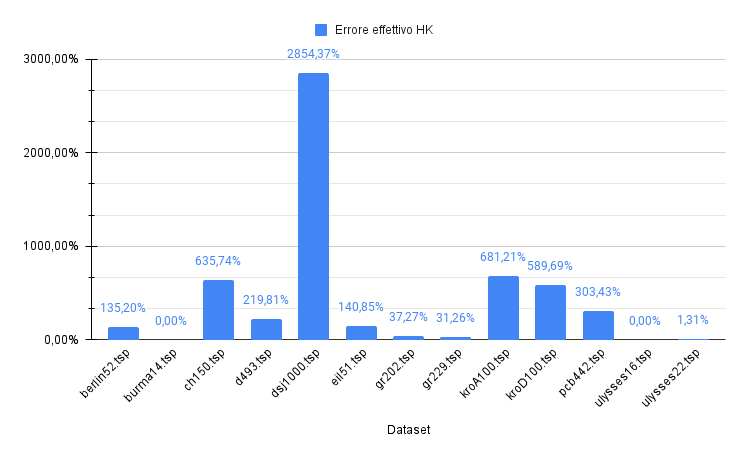
\includegraphics[width=0.85\textwidth]{res/images/errors/hk-effettivo.png}
	\caption{Errore effettivo dei risultati ottenuti con Held-Karp.}
	\label{fig:errors-hk-effettivo}
\end{figure}

\begin{figure}[H]
	\centering
	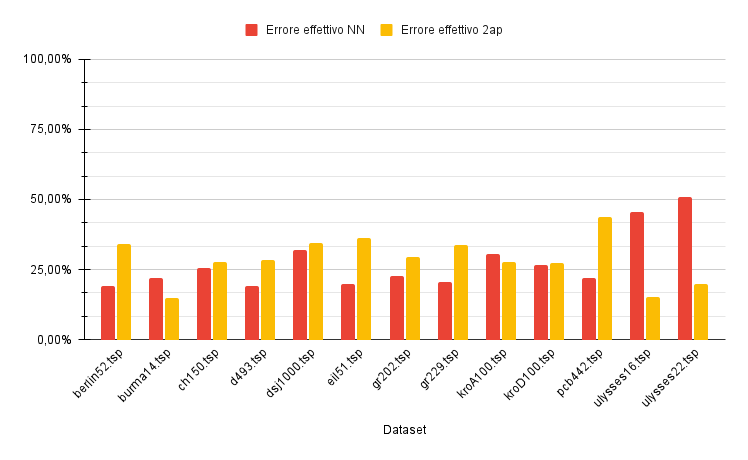
\includegraphics[width=0.85\textwidth]{res/images/errors/approx-effettivo.png}
	\caption{Errore effettivo dei risultati ottenuti con gli algoritmi non esatti.}
	\label{fig:errors-approx-effettivo}
\end{figure}

\begin{figure}[H]
	\centering
	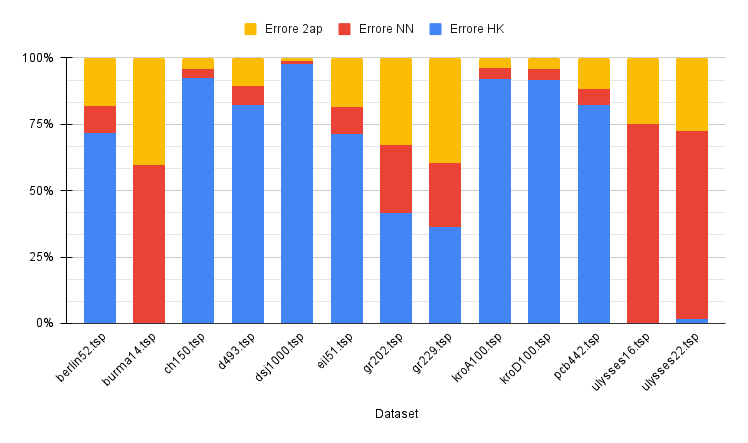
\includegraphics[width=0.85\textwidth]{res/images/errors/all.png}
	\caption{Errori in proporzione per i tre algoritmi.}
	\label{fig:errors-all}
\end{figure}

\begin{figure}[H]
	\centering
	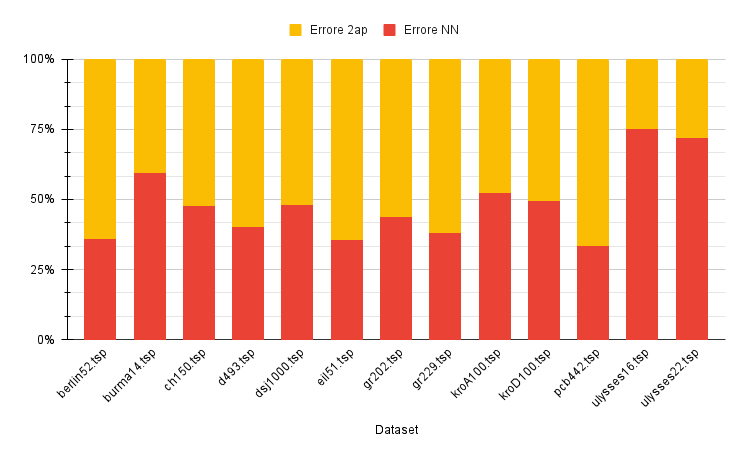
\includegraphics[width=0.85\textwidth]{res/images/errors/approx.png}
	\caption{Errori in proporzione per gli algoritmi non esatti.}
	\label{fig:errors-approx}
\end{figure}

Come si può evincere da questi grafici (fig. \ref{fig:errors-hk-effettivo}, \ref{fig:errors-approx-effettivo}, \ref{fig:errors-all}, \ref{fig:errors-approx}), l'algoritmo nearest neighbor sembra essere, \textit{in media}, più efficiente; ciò non è vero, però, per grafi più piccoli come \textit{burma14}, \textit{ulysses16} e \textit{ulysses22}, in cui l'algoritmo di 2-approssimazione si avvicina decisamente meglio alla soluzione ottima. 
Una possibile ipotesi che abbiamo avanzato nel corso dell'analisi di questi risultati potrebbe ricondursi alla natura \textit{greedy} dell'algoritmo nearest neighbor, che procede con la scelta ottima per ogni vertice incontrato. Pertanto, la potenzialità di questo algoritmo si riflette meglio con grafi di maggior dimensione proprio perché il numero di scelte da effettuare è maggiore e quindi il possibile tasso di errore si riduce in proporzione. Chiaramente questa ipotesi è puramente un'osservazione basata su nostre congetture che sarebbe interessante approfondire. 


\begin{figure}[H]
	\centering
	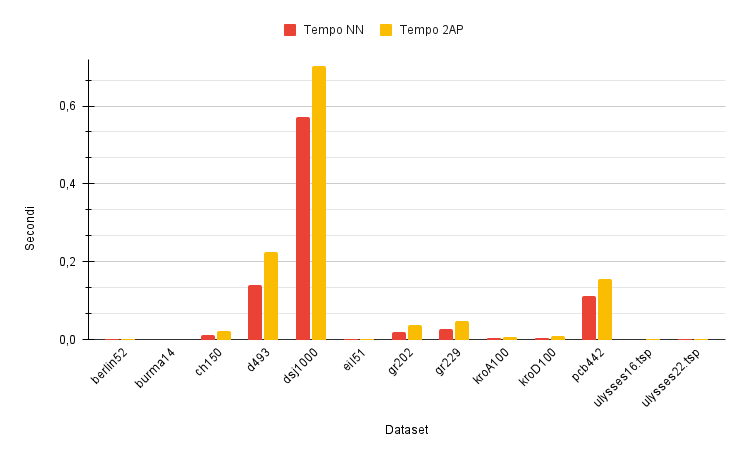
\includegraphics[width=1\textwidth]{res/images/time/time-nn-2ap.png}
	\caption{Tempi effettivi ottenuti con Nearest Neighbor e 2-approssimazione.}
	\label{fig:time-nn-2ap}
\end{figure}

Per quanto riguarda le tempistiche degli algoritmi di approssimazione, si può notare dal grafico \ref{fig:time-nn-2ap} che i tempi di esecuzione dei due algoritmi, anche ripetuti più e più volte, denotano un minore tempo di computazione effettivo per l'algoritmo di Nearest Neighbor, specialmente nei grafi più grandi. 
Analogamente, anche nei grafi di minore dimensione (fig. \ref{fig:time-detail-nn-2ap}) è possibile notare che questo algoritmo è quello che ci impiega meno tempo a livello computazionale, confermandosi quindi il più veloce dei tre. 

\begin{figure}[H]
	\centering
	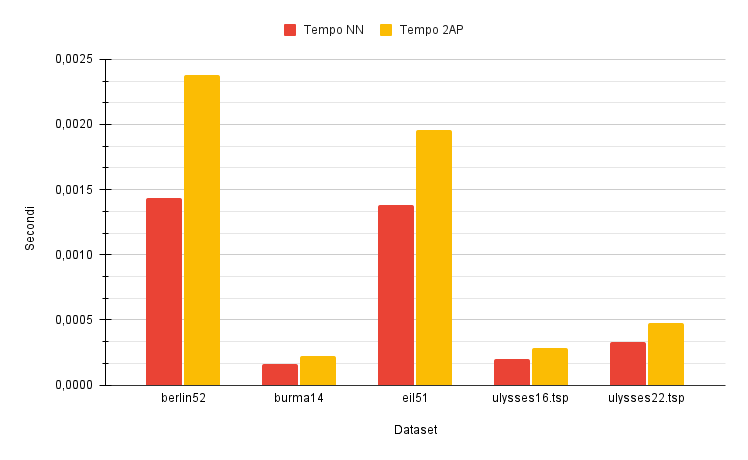
\includegraphics[width=1\textwidth]{res/images/time/time-detail-nn-2ap.png}
	\caption{Dettaglio dei tempi effettivi ottenuti con Nearest Neighbor e 2-approssimazione nei dataset più piccoli.}
	\label{fig:time-detail-nn-2ap}
\end{figure}

Per quanto concerne le tempistiche di Held and Karp, solo due dataset hanno computato il risultato entro tre minuti, mentre uno di questi, \textit{ulysses22}, ci è andato vicino con un errore del 1,31\% (fig. \ref{fig:errors-hk-effettivo}). Altri dataset, come \textit{burma14} e \textit{ulysses16}, hanno completato la computazione e hanno ottenuto in un tempo relativamente basso i risultati, rispettivamente di circa 0.35 e 1.96 secondi.

% Conclusioni belle
\newpage
\section{Conclusione}

% ottimizzazioni su naive molto utili --> risparmio di diverse chiamate a dfs / primi grafi molto veloci quasi quanto UF e prim

Alla fine del lavoro svolto possiamo dire che le ottimizzazioni che sono state implementate per la versione naive dell'algoritmo di Kruskal si sono 
rivelate utili per l'esecuzione dei primi grafi. Infatti,
\begin{enumerate}
    \item Il controllo dei \textit{self-loop} e della presenza o meno dei nodi dell'arco $(u, v)$ hanno permesso di risparmiare diverse chiamate a DFS per il 
    controllo della ciclicità del grafo $G$;
    \item La versione modificata di DFS permette di evitare la visita di tutto il grafo quando non è necessario. È sufficiente controllare che esista un cammino 
    da $u$ a $v$ nella componente connessa di $u$. Se tale cammino non esiste, allora il lato $(u, v)$ farà parte del MST $T$ finale.
\end{enumerate}
Queste ottimizzazioni hanno permesso di ottenere delle performance migliori nel momento in cui l'algoritmo inizia ad analizzare il grafo ricevuto in 
input. È possibile notare che i tempi per Kruskal Naive sono paragonabili ai tempi degli altri due algoritmi per grafi con un piccolo numero di vertici (cfr. \S{4.3}).


% ottimizzazione dello heap per Prim --> risparmio sulla ricerca lineare

In secondo luogo, per quanto riguarda l'implementazione della struttura dati Heap utilizzata per l'algoritmo di Prim abbiamo potuto constatare che l'ottimizzazione integrata attraverso una mappa che permettesse di salvare l'indice di posizione corrente nella lista ausiliaria ha ridotto di gran lunga la durata media dell'algoritmo di Prim, tendendo a essere più simile al tempo medio ottenuto da Kruskal Union Find. Questa miglioria ha permesso di accedere quindi in tempo costante ai singoli elementi della lista rimuovendo la complessità lineare, che precedentemente avrebbe reso computazionalmente più lento di un valore polinomiale l'algoritmo di Prim.


% misurazione più accurate 

Per quanto concerne le misurazioni effettuate abbiamo voluto rendere ciascuna misurazione il più preciso possibile così da ottenere risultati sui tempi medi di esecuzione più attendibili. Difatti, ripetendo l'esecuzione di ciascun grafo con tempo di esecuzione minore al secondo di un fattore \(k\), che rappresenta il numero di ripetizioni da eseguire per rientrare entro il secondo sulla base del tempo per una esecuzione, siamo riusciti ad avere un risultato più comparabile che ci ha permesso di fare dei confronti più interessanti (vedasi i risultati della sezione \S{4). 


% approccio di lavoro incrementale, ossia creo algoritmo, verifico efficacia (3 risultati uguali = risultati corretti), lo ottimizzo
Per quanto concerne il \textit{workflow} adottato all'interno del gruppo, avendo lavorato con un sistema di versionamento siamo riusciti ad organizzarci per realizzare e sviluppare attraverso un approccio incrementale ciascun algoritmo. Inizialmente infatti abbiamo iniziato con lo studiare bene il funzionamento di ogni algoritmo e poi, gradualmente, lo abbiamo implementato partendo dalle strutture dati richieste. Una volta controllato che in tutti e 3 i casi gli algoritmi ottenevano risultati identici sul peso finale degli archi, abbiamo ottimizzato ciascuno di essi limando sulle parti di codice superflue ed applicando delle migliorie in base a quanto il linguaggio Python ha da offrire. Infine, abbiamo voluto anche rendere facilmente utilizzabile l'applicazione finale, così da poter provare diversi dataset in diverse modalità. Per la realizzazione dei grafi, tuttavia, abbiamo preferito raccogliere i risultati e generare i grafici sfruttando Google Colab, la cui logica è stata riportata per completezza all'interno di una cartella del progetto (\textit{graph-generation}).


% tiriamo le somme sui risultati 

In linea di massima siamo stati contenti dei risultati ottenuti sebbene l'uso del linguaggio Python, pur se relativamente semplice, ci è risultato abbastanza disordinato per la mancanza di \textit{strong typing}, cosa che ci ha causato inizialmente diversi rallentamenti nello sviluppo degli algoritmi.
Per concludere, quanto ci è risultato per gli algoritmi è in linea con quanto ci aspettavamo, difatti: 
\begin{itemize}
    \item Kruskal Naive risulta il più lento tra i tre algoritmi e il meno efficiente in termini di tempo medio di esecuzione per grafi con molti nodi;
    \item Kruskal Union Find risulta il più veloce e il più efficiente tra i tre algoritmi, specialmente con grafi di grandi dimensioni;
    \item Prim si può classificare in secondo posto rispetto a Kruskal Union Find, avendo un tempo di esecuzione sufficientemente buono anche per grafi di grandi dimensioni. 
\end{itemize}





% Appendice
\newpage
\begin{appendices}

   \section{Appendice}

\subsection{Risultati output Stoer e Wagner}

\subsection{Risultati output Karger e Stein}

\end{appendices}